\documentclass[
	openboth, % Capítulos começam em página direita
	oneside,   % Impressão frente e verso
	a4paper,   % Tamanho do papel
	english,   % Idioma adiciona para hifenizaçãoo
	brazil     % O ultimo é o idioma principal
]{abntex2}

\usepackage{lmodern}                               % Usa família de fontes Latin Modern
\usepackage[T1]{fontenc}                           % Codifição Type1 para a fonte (Fontes de 8 bits para incluir as fontes do alfabeto brasileiro)
\usepackage[UTF8]{inputenc}                        % Codificação unicode "UTF8"
\usepackage{microtype}                             % Melhorias na justificação (Evita bad/underfullbox)
\usepackage{indentfirst}                           % Indenta o primeiro parágrafo da seção
\usepackage{amssymb}                               % Símbolos matemáticos
\usepackage{enumitem}                              % Melhoria no suporte aos ambientes de numeração
\usepackage{color}                                 % Suporte a cores
\definecolor{blue}{RGB}{41,5,195}                  % Alterando o aspécto da cor Azul
\usepackage{graphicx}                              % Suporte a gráficos e figuras
\usepackage[alf]{abntex2cite}                      % Citações no padrão ABNT

% informações do PDF
\makeatletter
\hypersetup{
	%pagebackref=true,
	pdftitle={\@title}, 
	pdfauthor={\@author},
	pdfsubject={\imprimirpreambulo},
	pdfcreator={LaTeX with abnTeX2},
	pdfkeywords={abnt}{latex}{abntex}{abntex2}{trabalho acadêmico}, 
	colorlinks=true,       		% false: boxed links; true: colored links
	linkcolor=black,          	% color of internal links
	citecolor=black,        		% color of links to bibliography
	filecolor=black,      		% color of file links
	urlcolor=black,
	bookmarksdepth=4
}
\makeatother

% O tamanho do parágrafo é dado por:
\setlength{\parindent}{1.3cm}

% Controle do espaçamento entre um parágrafo e outro:
\setlength{\parskip}{0.2cm}  % tente também \onelineskip





\makeindex
\makeglossary


\AtBeginDocument{
	\pagenumbering{gobble}
	\frenchspacing 
	\pretextual
	\tableofcontents*
	\textual
}

\begin{document}
	\chapter{Introdução}
	\pagenumbering{arabic}
	\setcounter{page}{1}
	
	As preocupações devido às emissões de CO2 tornaram a utilização de fontes de energias renováveis interessantes. Dentre elas, a energia baseada no vento se mostrou bastante promissora, pois o Brasil tem um dos maiores potenciais eólicos do mundo \cite{atlaseolico}.
	
	Com o aumento da participação da matriz eólica surgem novos desafios. A velocidade do vento é uma grandeza com grande variação instantânea, podendo variar bastante em questão de horas ou, até mesmo minutos. Essa variação, se não for contornada, pode trazer problemas de qualidade de energia, como a variação da frequência da rede devido a variação do vento, principalmente em redes mais fracas e dependentes da energia eólica. Além disso, há a presença de harmônicos devido ao movimento caótico do vento e ao efeito de sombra, ou seja, a perda de potência no momento em que uma das pás passa pela torre \cite{pintofundamentos}.
	
	Uma das soluções para melhorar a qualidade de energia de fontes eólicas é uso da eletrônica de potência em conjunto com topologias alternativas de geradores, como o GIDA (Gerador de indução duplamente alimentado).  A escolha do GIDA ocorre devido ao seu conversor processar até 30\% da potência nominal do gerador, enquanto em outros geradores com conversor acoplado esse valor chega a 100\%. Isto possibilita a redução do custo do conversor \cite{dattacomparacao,simoesrenewableinduction}. Nessa configuração tanto o estator quanto o rotor estão conectados à rede. Sendo o primeiro conectado diretamente (Figura \ref{figura:gida_esquematico} - A) e o rotor  é conectado através de uma derivação (Figura \ref{figura:gida_esquematico} - C), no qual existe um conversor CA/CA bidirecional \emph{back-to-back} \cite{heliodfig}.
	
	
	\begin{figure}[h]
		\centering
		\label{figura:gida_esquematico}
		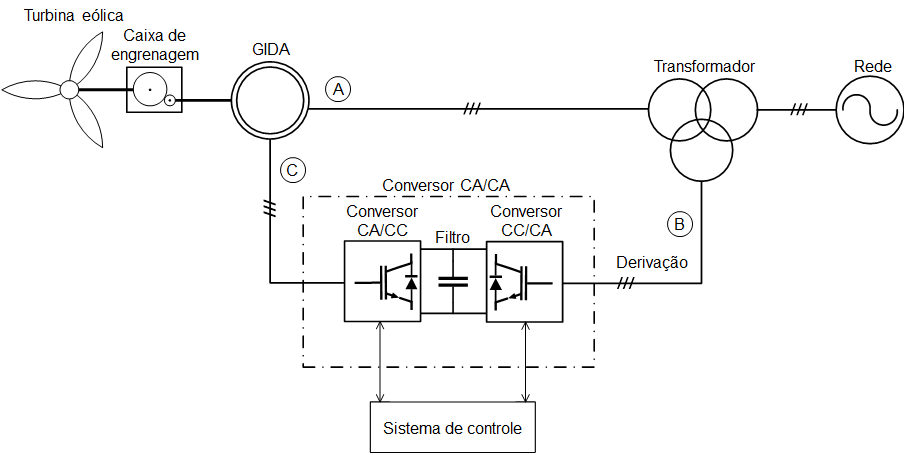
\includegraphics[width=1\textwidth]{Figuras/gida_esquematico.png}
		\caption{Esquema do GIDA conectado à  rede para geração de energia eólica (Próprio autor)}
	\end{figure}

	O conversor back to back é dividido em dois estágios. O primeiro converte a tensão alternada do lado voltado para a rede (Figura \ref{figura:gida_esquematico} - B) em tensão contínua, que é feita através do processo de retificação e com a ajuda de um filtro capacitivo, localizado logo após a saída deste estágio. Já o segundo estágio converte a tensão contínua novamente em tensão alternada, dessa vez aplicada ao rotor (Figura \ref{figura:gida_esquematico} - C). Esse processo é feito através da modulação por largura de pulso (PWM). Ambos os estágios são constituídos por pontes de \emph{Insulated Gate Bipolar Transistor} (IGBT), que são chaves semicondutoras para médias tensões. Dependendo de como as pontes de IGBT são chaveadas é possível regular a saída do conversor para tensões e frequências específicas \cite{alfeu}. 
	
	As técnicas de controle vetorial por orientação do fluxo do estator, ou de rotor, ou tensão de estator, permitem controlar separadamente as potências ativas e reativas do GIDA, além das grandezas de tensão e frequência. Essas técnicas consistem em controlar as componentes de eixo direto e em quadratura das correntes do rotor. Inicialmente, utilizavam-se controladores proporcionais-integrais (PI) [ref] para este fim. Mais recentemente, com o avanço dos sistemas computacionais e das técnicas de controle digital, surgiram novas alternativas como o deadbeat [ref], controle preditivo de matriz dinâmica de controle (DMC), controle preditivo baseado em modelo (CPBM) [ref] e controle preditivo generalizado (GPC) [ref]. Todas elas apresentam excelente desempenho, porém a maioria dos trabalhos encontrados na literatura se limitam apenas a simulação. Este trabalho tem o objetivo de preencher a lacuna existente na implementação desses tipos de controladores. Para isso será implementado o controlador MAC aplicado as potências ativas e reativas, proposto por (Referência), no kit de GIDA de um dos laboratório de pós-graduação da UFABC (Nome do laboratório).

	
	\bibliographystyle{abntex2-alf}
	\bibliography{biblio}
\end{document}